% Options for packages loaded elsewhere
\PassOptionsToPackage{unicode}{hyperref}
\PassOptionsToPackage{hyphens}{url}
%
\documentclass[
  ignorenonframetext,
]{beamer}
\usepackage{pgfpages}
\setbeamertemplate{caption}[numbered]
\setbeamertemplate{caption label separator}{: }
\setbeamercolor{caption name}{fg=normal text.fg}
\beamertemplatenavigationsymbolsempty
% Prevent slide breaks in the middle of a paragraph
\widowpenalties 1 10000
\raggedbottom
\setbeamertemplate{part page}{
  \centering
  \begin{beamercolorbox}[sep=16pt,center]{part title}
    \usebeamerfont{part title}\insertpart\par
  \end{beamercolorbox}
}
\setbeamertemplate{section page}{
  \centering
  \begin{beamercolorbox}[sep=12pt,center]{part title}
    \usebeamerfont{section title}\insertsection\par
  \end{beamercolorbox}
}
\setbeamertemplate{subsection page}{
  \centering
  \begin{beamercolorbox}[sep=8pt,center]{part title}
    \usebeamerfont{subsection title}\insertsubsection\par
  \end{beamercolorbox}
}
\AtBeginPart{
  \frame{\partpage}
}
\AtBeginSection{
  \ifbibliography
  \else
    \frame{\sectionpage}
  \fi
}
\AtBeginSubsection{
  \frame{\subsectionpage}
}
\usepackage{amsmath,amssymb}
\usepackage{iftex}
\ifPDFTeX
  \usepackage[T1]{fontenc}
  \usepackage[utf8]{inputenc}
  \usepackage{textcomp} % provide euro and other symbols
\else % if luatex or xetex
  \usepackage{unicode-math} % this also loads fontspec
  \defaultfontfeatures{Scale=MatchLowercase}
  \defaultfontfeatures[\rmfamily]{Ligatures=TeX,Scale=1}
\fi
\usepackage{lmodern}
\usetheme[]{Madrid}
\ifPDFTeX\else
  % xetex/luatex font selection
\fi
% Use upquote if available, for straight quotes in verbatim environments
\IfFileExists{upquote.sty}{\usepackage{upquote}}{}
\IfFileExists{microtype.sty}{% use microtype if available
  \usepackage[]{microtype}
  \UseMicrotypeSet[protrusion]{basicmath} % disable protrusion for tt fonts
}{}
\makeatletter
\@ifundefined{KOMAClassName}{% if non-KOMA class
  \IfFileExists{parskip.sty}{%
    \usepackage{parskip}
  }{% else
    \setlength{\parindent}{0pt}
    \setlength{\parskip}{6pt plus 2pt minus 1pt}}
}{% if KOMA class
  \KOMAoptions{parskip=half}}
\makeatother
\usepackage{xcolor}
\newif\ifbibliography
\usepackage{color}
\usepackage{fancyvrb}
\newcommand{\VerbBar}{|}
\newcommand{\VERB}{\Verb[commandchars=\\\{\}]}
\DefineVerbatimEnvironment{Highlighting}{Verbatim}{commandchars=\\\{\}}
% Add ',fontsize=\small' for more characters per line
\usepackage{framed}
\definecolor{shadecolor}{RGB}{248,248,248}
\newenvironment{Shaded}{\begin{snugshade}}{\end{snugshade}}
\newcommand{\AlertTok}[1]{\textcolor[rgb]{0.94,0.16,0.16}{#1}}
\newcommand{\AnnotationTok}[1]{\textcolor[rgb]{0.56,0.35,0.01}{\textbf{\textit{#1}}}}
\newcommand{\AttributeTok}[1]{\textcolor[rgb]{0.13,0.29,0.53}{#1}}
\newcommand{\BaseNTok}[1]{\textcolor[rgb]{0.00,0.00,0.81}{#1}}
\newcommand{\BuiltInTok}[1]{#1}
\newcommand{\CharTok}[1]{\textcolor[rgb]{0.31,0.60,0.02}{#1}}
\newcommand{\CommentTok}[1]{\textcolor[rgb]{0.56,0.35,0.01}{\textit{#1}}}
\newcommand{\CommentVarTok}[1]{\textcolor[rgb]{0.56,0.35,0.01}{\textbf{\textit{#1}}}}
\newcommand{\ConstantTok}[1]{\textcolor[rgb]{0.56,0.35,0.01}{#1}}
\newcommand{\ControlFlowTok}[1]{\textcolor[rgb]{0.13,0.29,0.53}{\textbf{#1}}}
\newcommand{\DataTypeTok}[1]{\textcolor[rgb]{0.13,0.29,0.53}{#1}}
\newcommand{\DecValTok}[1]{\textcolor[rgb]{0.00,0.00,0.81}{#1}}
\newcommand{\DocumentationTok}[1]{\textcolor[rgb]{0.56,0.35,0.01}{\textbf{\textit{#1}}}}
\newcommand{\ErrorTok}[1]{\textcolor[rgb]{0.64,0.00,0.00}{\textbf{#1}}}
\newcommand{\ExtensionTok}[1]{#1}
\newcommand{\FloatTok}[1]{\textcolor[rgb]{0.00,0.00,0.81}{#1}}
\newcommand{\FunctionTok}[1]{\textcolor[rgb]{0.13,0.29,0.53}{\textbf{#1}}}
\newcommand{\ImportTok}[1]{#1}
\newcommand{\InformationTok}[1]{\textcolor[rgb]{0.56,0.35,0.01}{\textbf{\textit{#1}}}}
\newcommand{\KeywordTok}[1]{\textcolor[rgb]{0.13,0.29,0.53}{\textbf{#1}}}
\newcommand{\NormalTok}[1]{#1}
\newcommand{\OperatorTok}[1]{\textcolor[rgb]{0.81,0.36,0.00}{\textbf{#1}}}
\newcommand{\OtherTok}[1]{\textcolor[rgb]{0.56,0.35,0.01}{#1}}
\newcommand{\PreprocessorTok}[1]{\textcolor[rgb]{0.56,0.35,0.01}{\textit{#1}}}
\newcommand{\RegionMarkerTok}[1]{#1}
\newcommand{\SpecialCharTok}[1]{\textcolor[rgb]{0.81,0.36,0.00}{\textbf{#1}}}
\newcommand{\SpecialStringTok}[1]{\textcolor[rgb]{0.31,0.60,0.02}{#1}}
\newcommand{\StringTok}[1]{\textcolor[rgb]{0.31,0.60,0.02}{#1}}
\newcommand{\VariableTok}[1]{\textcolor[rgb]{0.00,0.00,0.00}{#1}}
\newcommand{\VerbatimStringTok}[1]{\textcolor[rgb]{0.31,0.60,0.02}{#1}}
\newcommand{\WarningTok}[1]{\textcolor[rgb]{0.56,0.35,0.01}{\textbf{\textit{#1}}}}
\usepackage{graphicx}
\makeatletter
\def\maxwidth{\ifdim\Gin@nat@width>\linewidth\linewidth\else\Gin@nat@width\fi}
\def\maxheight{\ifdim\Gin@nat@height>\textheight\textheight\else\Gin@nat@height\fi}
\makeatother
% Scale images if necessary, so that they will not overflow the page
% margins by default, and it is still possible to overwrite the defaults
% using explicit options in \includegraphics[width, height, ...]{}
\setkeys{Gin}{width=\maxwidth,height=\maxheight,keepaspectratio}
% Set default figure placement to htbp
\makeatletter
\def\fps@figure{htbp}
\makeatother
\setlength{\emergencystretch}{3em} % prevent overfull lines
\providecommand{\tightlist}{%
  \setlength{\itemsep}{0pt}\setlength{\parskip}{0pt}}
\setcounter{secnumdepth}{-\maxdimen} % remove section numbering
\logo{
\includegraphics[height=1cm,width=3cm]{logo.png}}
\usetheme{Madrid}
\usefonttheme{serif}
\setbeamertemplate{navigation symbols}{}

\usepackage{amsmath}



\ifLuaTeX
  \usepackage{selnolig}  % disable illegal ligatures
\fi
\IfFileExists{bookmark.sty}{\usepackage{bookmark}}{\usepackage{hyperref}}
\IfFileExists{xurl.sty}{\usepackage{xurl}}{} % add URL line breaks if available
\urlstyle{same}
\hypersetup{
  pdftitle={Leksioni1},
  pdfauthor={Endri Raco},
  hidelinks,
  pdfcreator={LaTeX via pandoc}}

\title{Leksioni1}
\author{Endri Raco}
\date{21 April, 2024}

\begin{document}
\frame{\titlepage}

\begin{frame}[allowframebreaks]
  \tableofcontents[hideallsubsections]
\end{frame}
\begin{frame}{Organizimi i kursit - Python}
\protect\hypertarget{organizimi-i-kursit---python}{}
\begin{itemize}
\item
  Instalimi i Python
\item
  Konceptet bazë të programimit në Python
\item
  Analizimi i të dhënave me Python
\item
  Vizualizimi i të dhënave në Python
\end{itemize}
\end{frame}

\begin{frame}{Organizimi i kursit - Python dhe GIS}
\protect\hypertarget{organizimi-i-kursit---python-dhe-gis}{}
\begin{itemize}
\item
  Procesimi i të dhënave vektor
\item
  Procesimi i të dhënave raster
\item
  Vizualizimi i të dhënave gjeografike
\item
  Lidhja me burimet gjeografike online
\end{itemize}
\end{frame}

\begin{frame}{Organizimi i kursit - Python dhe GIS}
\protect\hypertarget{organizimi-i-kursit---python-dhe-gis-1}{}
\begin{itemize}
\item
  Interpolimi hapësinor
\item
  Analiza e rrjetit hapësinor
\item
  Analiza e terrenit
\end{itemize}
\end{frame}

\begin{frame}{Instalimi i Python-it}
\protect\hypertarget{instalimi-i-python-it}{}
\begin{itemize}
\item
  Python dhe libraritë e tij mund të instalohen lehtësisht duke përdorur
  paketa të ndryshme.
\item
  Për të instaluar Python-in, \textbf{Miniconda} është një zgjedhje e
  mirë sepse ofron një mjedis të qëndrueshëm dhe mënjanon konfliktin e
  librarive.
\end{itemize}
\end{frame}

\begin{frame}{Menaxhimi i Varësive midis librarive (dependency)}
\protect\hypertarget{menaxhimi-i-varuxebsive-midis-librarive-dependency}{}
\begin{itemize}
\item
  Python ka një numër të madh librarish të disponueshme që mund të kenë
  varësi të ndërsjella.
\item
  Është e rëndësishme që libraritë dhe versionet e tyre të punojnë mirë
  së bashku.
\item
  Menaxhimi i librarive (package managers)
\end{itemize}
\end{frame}

\begin{frame}{Pluset e përdorimit të Miniconda}
\protect\hypertarget{pluset-e-puxebrdorimit-tuxeb-miniconda}{}
\begin{itemize}
\item
  Miniconda përfshin një menaxher librarish që lehtëson instalimin dhe
  përditësimin.
\item
  Ka support shumë të mirë
\item
  Falas
\item
  Ofron ndërfaqe grafike për lehtësi përdorimi
\end{itemize}
\end{frame}

\begin{frame}{Mjediset Virtuale (Virtual environments)}
\protect\hypertarget{mjediset-virtuale-virtual-environments}{}
\begin{itemize}
\item
  Mjediset virtuale krijojnë një hapësirë të izoluar për projektet tona
  Python.
\item
  Krijimi i mjediseve virtuale ndihmon për të shmangur konfliktet midis
  librarive dhe instalimeve të ndryshme.
\item
  Mund të krijojmë mjedise të shumta dhe të kalojmë lehtësisht mes tyre.
\end{itemize}
\end{frame}

\begin{frame}{Konfigurimi dhe Dokumentimi i Mjediseve}
\protect\hypertarget{konfigurimi-dhe-dokumentimi-i-mjediseve}{}
\begin{itemize}
\item
  Përdorim skedarët \textbf{YAML} për të dokumentuar konfigurimet e
  mjediseve që krijojmë.
\item
  Në skedarët YAML, mund të përcaktojmë specifikat e mjedisit, përfshirë
  versionin e Python-it dhe libraritë që do përdorim.
\item
  Formati tipik për mjediset Conda/Mamba është \textbf{environment.yaml}
\end{itemize}
\end{frame}

\begin{frame}{Praktika të Mira}
\protect\hypertarget{praktika-tuxeb-mira}{}
\begin{itemize}
\tightlist
\item
  Është një praktikë e mirë të instalojmë të gjitha libraritë (kur është
  e mundur) nga i njëjti kanal Conda, si p.sh., \textbf{conda-forge},
  dhe të mos përziejmë \textbf{Conda} dhe \textbf{Pip} për instalime
  nëse nuk është e domosdoshme.
\end{itemize}
\end{frame}

\begin{frame}{Çfarë është një Kanal Conda}
\protect\hypertarget{uxe7faruxeb-uxebshtuxeb-njuxeb-kanal-conda}{}
\begin{itemize}
\item
  Një kanal Conda është një vendndodhje/server me një adresë të dedikuar
  në internet, ku ruhen libraritë.
\item
  Kanali shërben si bazë për strehimin(repository) e librarive, dhe
  menaxherët e paketave (si Conda/Mamba) kërkojnë dhe shkarkojnë
  libraritë nga këto kanale.
\end{itemize}
\end{frame}

\begin{frame}{Instalimi i Python dhe i librarive të rekomanduara}
\protect\hypertarget{instalimi-i-python-dhe-i-librarive-tuxeb-rekomanduara}{}
\textbf{Windows:}

\begin{itemize}
\tightlist
\item
  Shkarkojmë versionin Miniconda të bazuar në Python 3 që është i
  përshtatshëm për sistemin operativ ku do punojmë.
\end{itemize}

\url{https://docs.conda.io/en/latest/miniconda.html\#latest-miniconda-installer-links}

\begin{itemize}
\tightlist
\item
  Ndjekim udhëzimet e instalimit nga faqja e Miniconda.
\end{itemize}
\end{frame}

\begin{frame}{Kontrolli i instalimit}
\protect\hypertarget{kontrolli-i-instalimit}{}
\begin{itemize}
\tightlist
\item
  Hapim \textbf{Terminalin} ose \textbf{Anaconda Prompt}
\end{itemize}

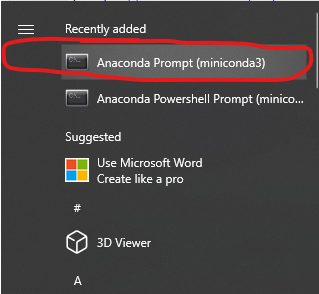
\includegraphics{./Figs/anac_prompt.png}
\end{frame}

\begin{frame}{Kontrolli i instalimit}
\protect\hypertarget{kontrolli-i-instalimit-1}{}
\begin{itemize}
\tightlist
\item
  Për të siguruar që conda është instaluar siç duhet, ekzekutojmë
  komandën:
\end{itemize}

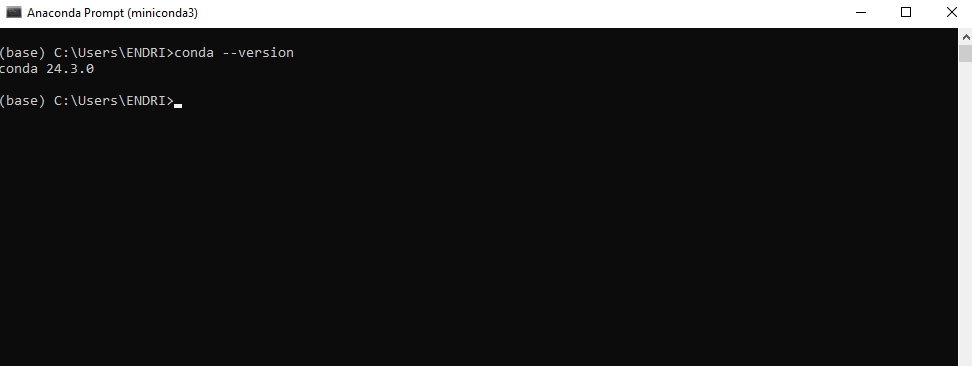
\includegraphics{./Figs/conda_ver.png}
\end{frame}

\begin{frame}[fragile]{Instalimi i Mamba}
\protect\hypertarget{instalimi-i-mamba}{}
\begin{itemize}
\item
  Mamba është një menaxher librarish për Miniconda.
\item
  Për të instaluar \textbf{mamba}, hapim \textbf{Terminalin} ose
  \textbf{Command Prompt} në Windows si administrator.
\item
  Ekzekutojmë komandën:
\end{itemize}

\begin{Shaded}
\begin{Highlighting}[]
\NormalTok{  conda install mamba {-}n base {-}c conda{-}forge}
\end{Highlighting}
\end{Shaded}
\end{frame}

\end{document}
